% =====================================================================
%  Case Study 2 — Agent A/B : Simulating Large-Scale A/B Testing
%  Frames only. \input this right AFTER the existing
%    \section[Case Study 2: Simulating Large-Scale A/B Testing ...]{...}
%  line in user-simulator.tex.
%  Figures live in figures/agentab/ (paper figures + GPT motivation art).
% =====================================================================

% ---- Bridge from UXAgent: small scale -> can it scale? ----
\begin{frame}[standout]
  UXAgent: LLM agents simulate users at \emph{small scale} to help UX researchers.
  \vspace{10pt}
  \pause

  But real design decisions ship through \emph{large-scale A/B testing}.
  \vspace{6pt}

  Can simulated users \ul{scale up}?
\end{frame}

\begin{frame}[plain]
  \begin{figure}[htp]
    \centering
    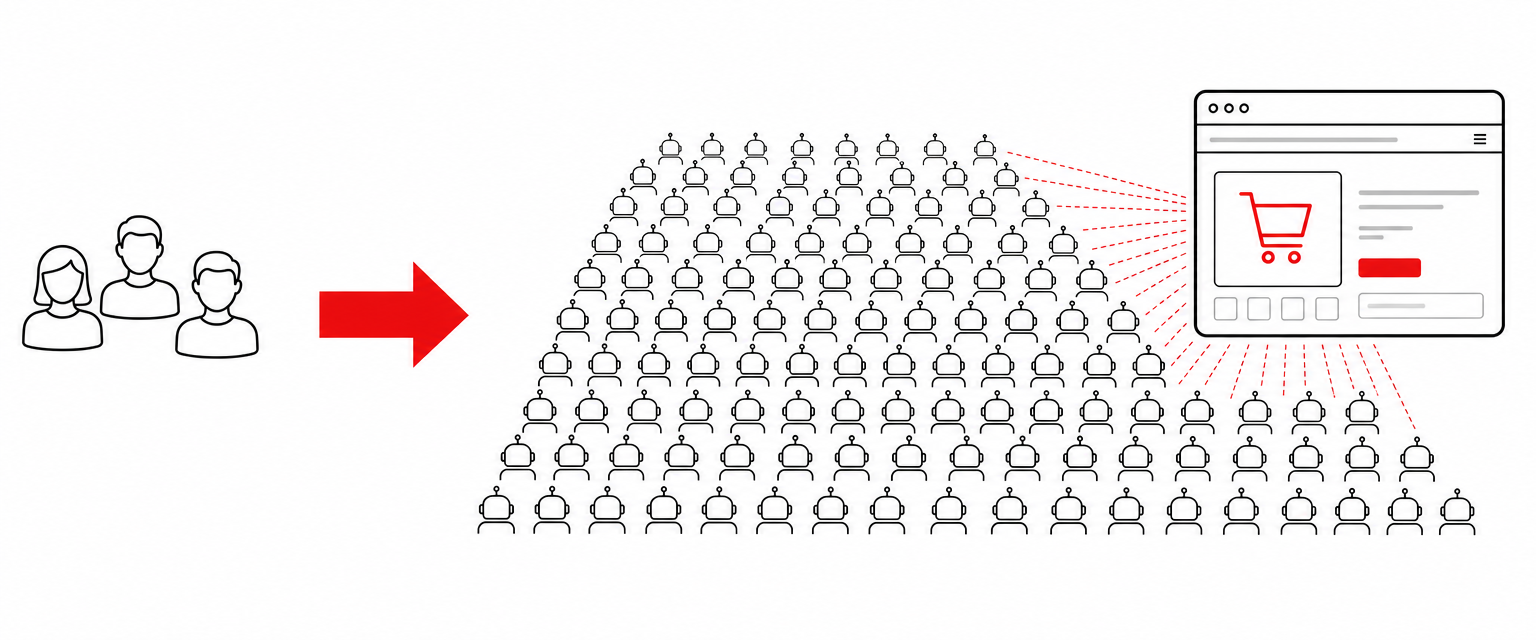
\includegraphics[width=\linewidth]{figures/agentab/scale_concept.png}
  \end{figure}
\end{frame}

% ---- What A/B testing is, and why it is heavy ----
\begin{frame}{Three Bottlenecks in A/B Testing}
  \begin{figure}[htp]
    \centering
    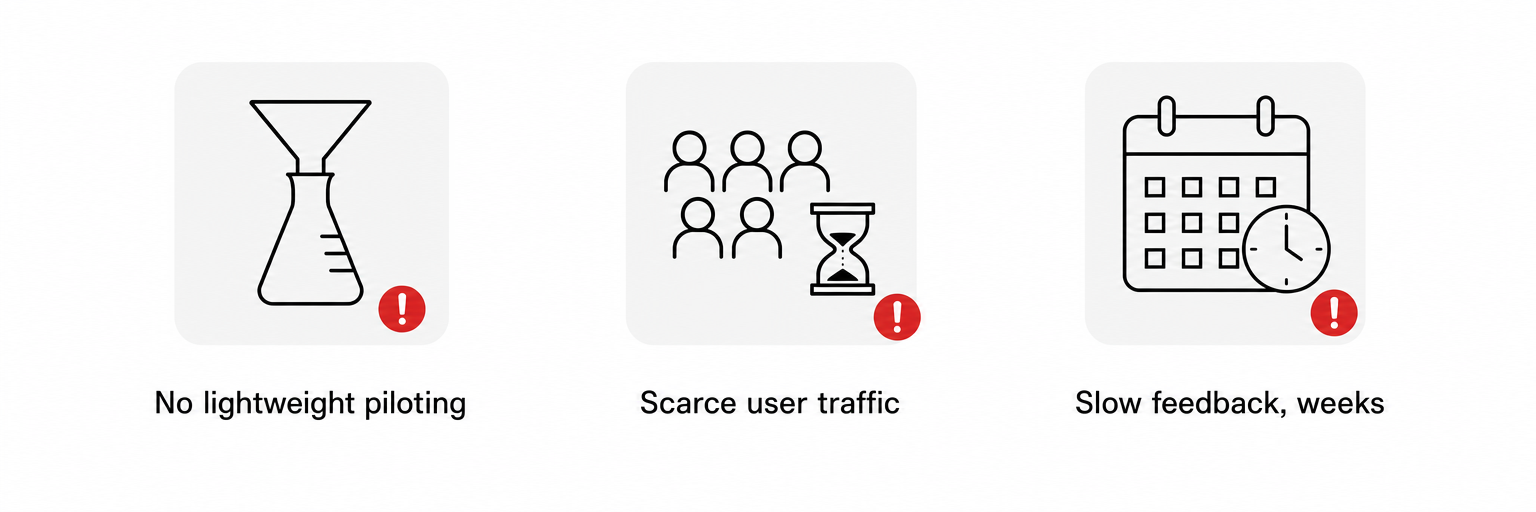
\includegraphics[width=\linewidth]{figures/agentab/bottlenecks.png}
  \end{figure}
  \centering\small From a formative study with 6 A/B-testing practitioners --- many promising ideas never get piloted before launch.
\end{frame}

% ---- The question ----
\begin{frame}[standout]
  Can we deploy \textbf{thousands} of persona-driven LLM agents on the \emph{live} website
  \vspace{6pt}

  --- to pilot an A/B test \ul{before} spending real user traffic?
\end{frame}

% ---- System overview ----
\begin{frame}{Our Solution: Agent A/B}
  \begin{figure}[htp]
    \centering
    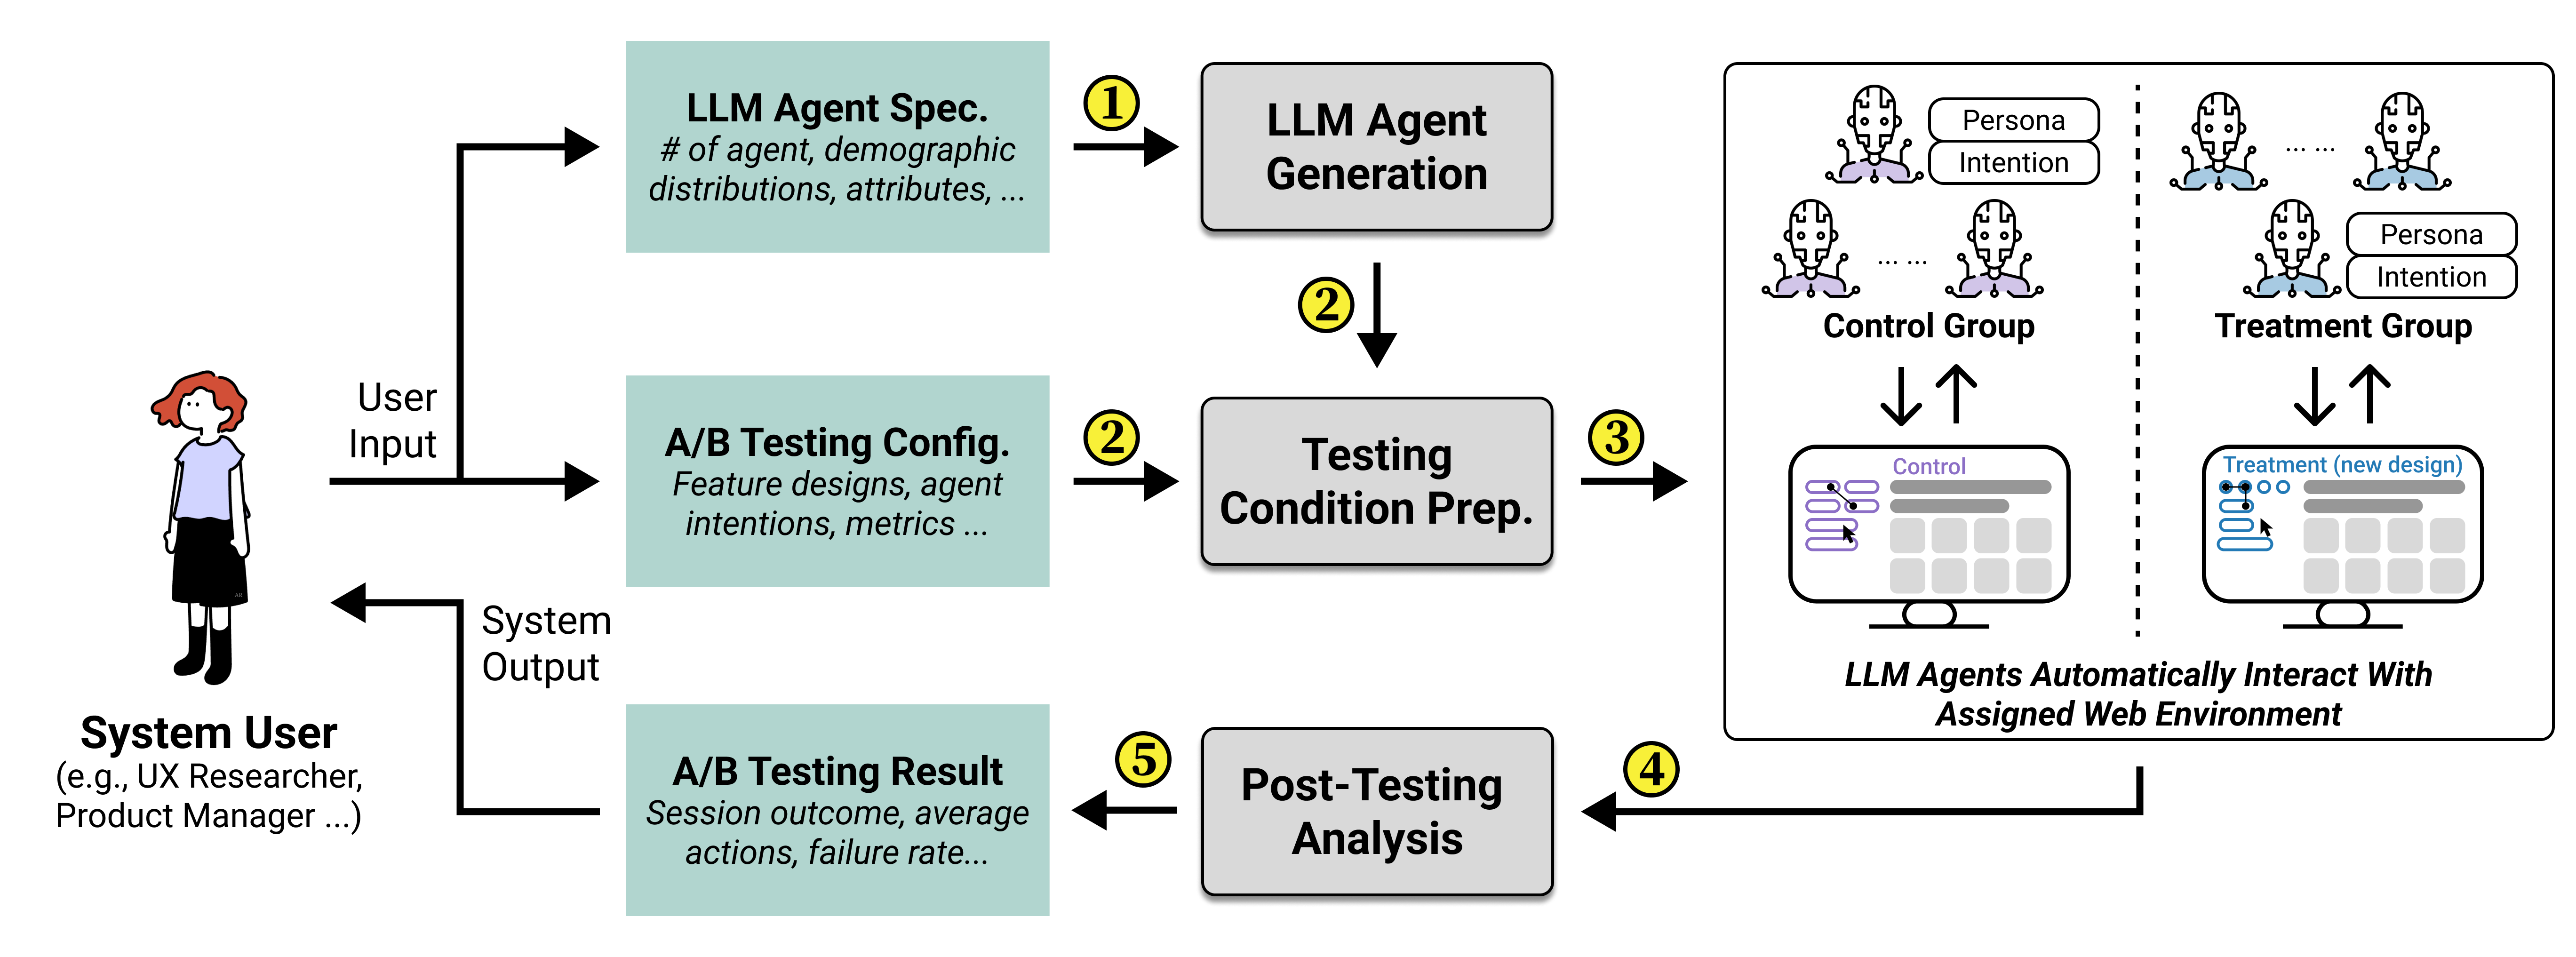
\includegraphics[width=\linewidth]{figures/agentab/abtest.png}
  \end{figure}
  \centering\small Plug-and-play with existing agent stacks (Claude computer-use, ReAct).
\end{frame}

% \begin{frame}{Inside One Agent}
%   \begin{figure}[htp]
%     \centering
%     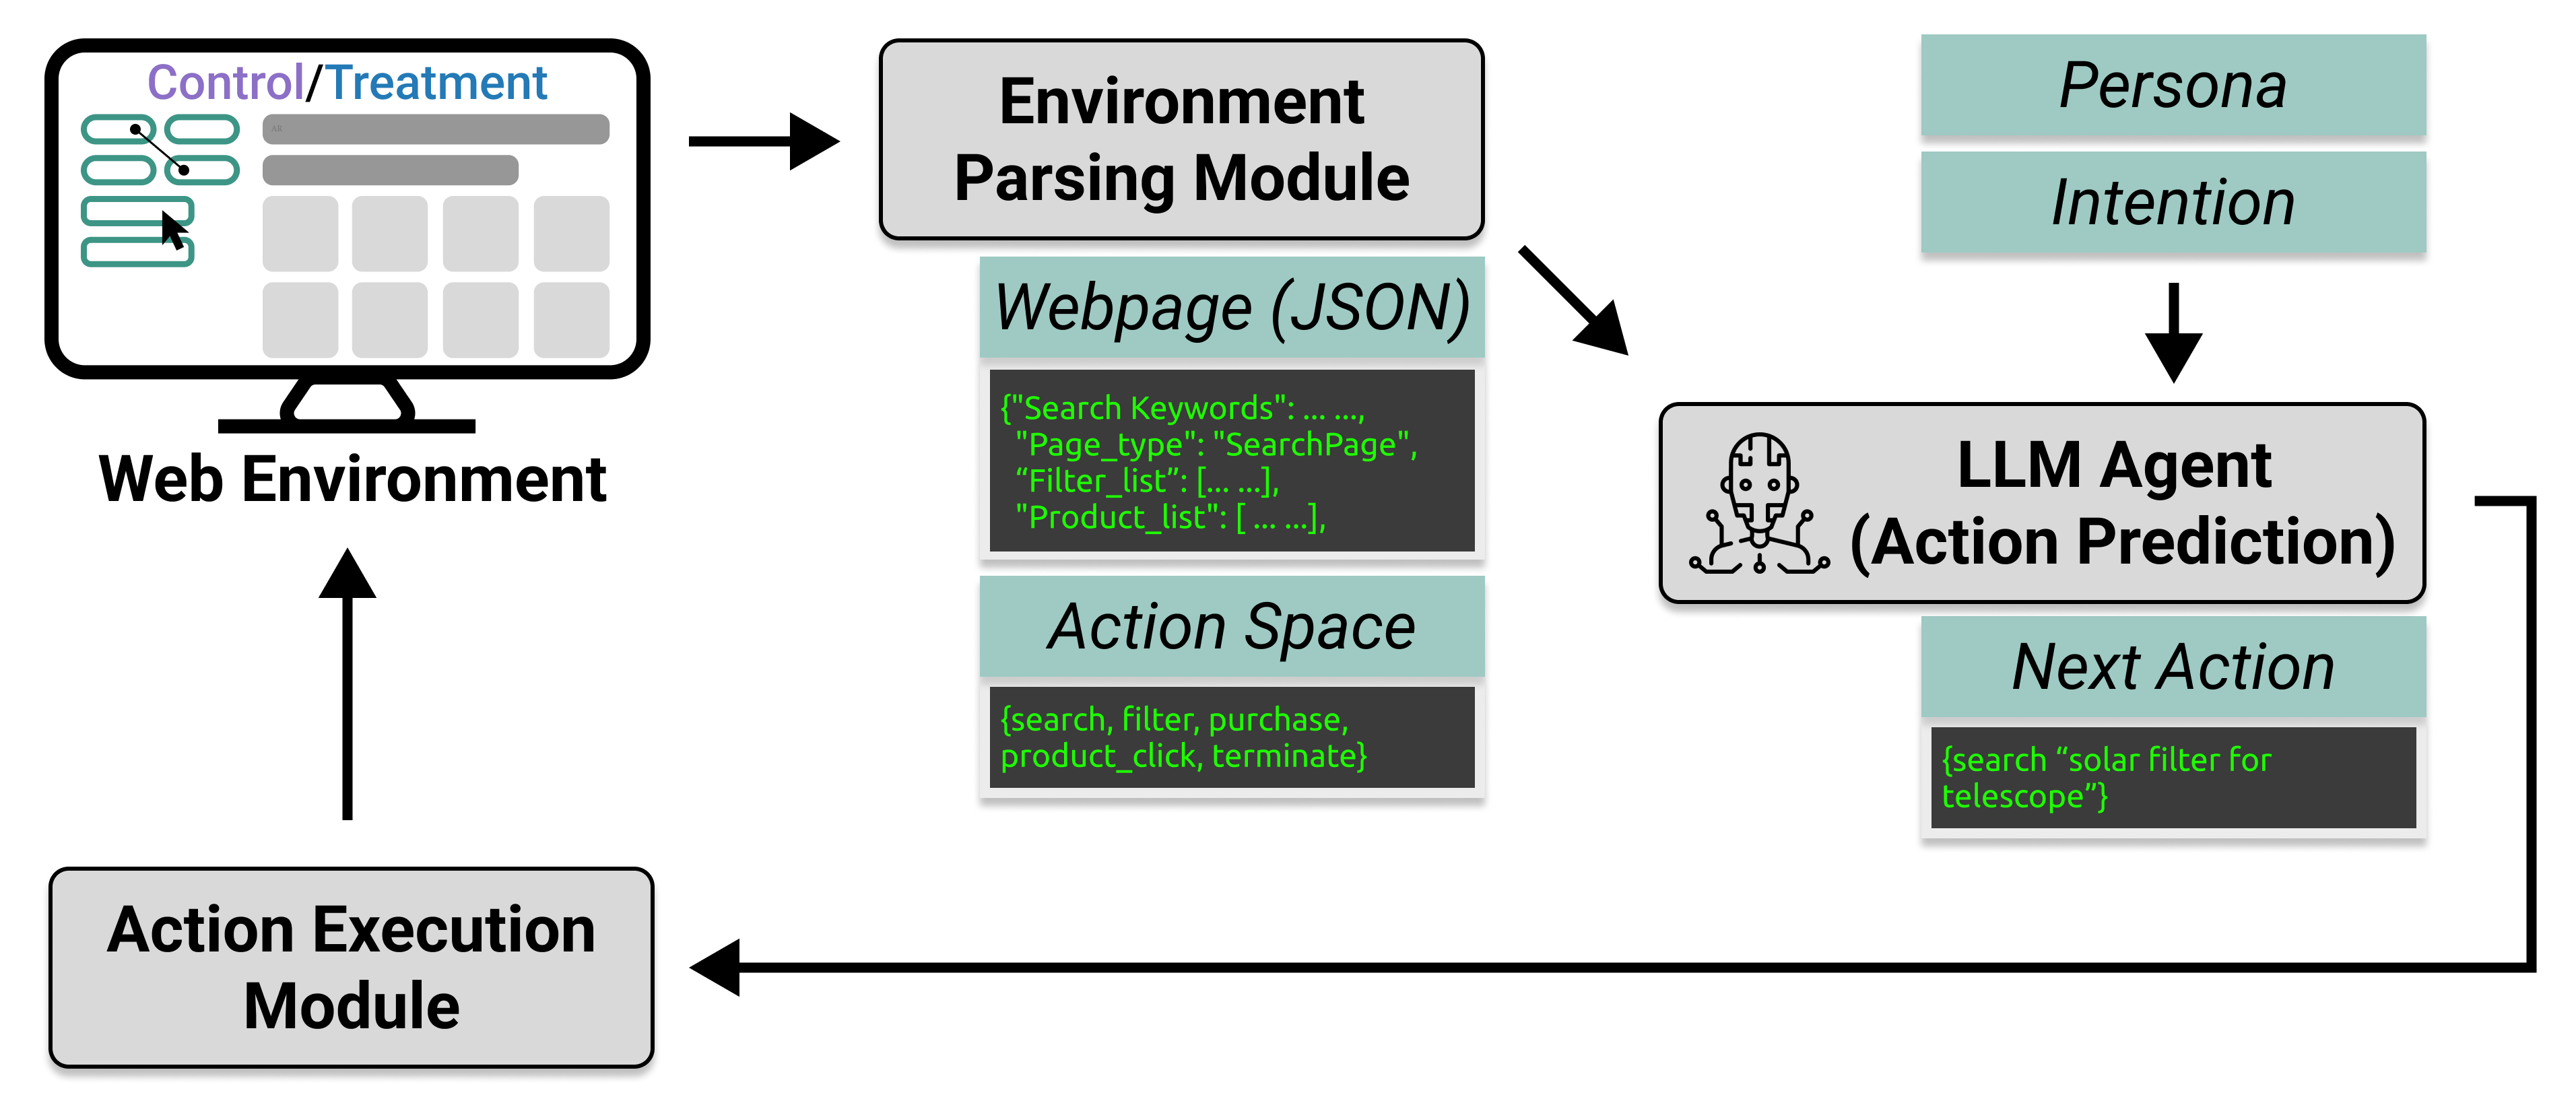
\includegraphics[width=.96\linewidth]{figures/agentab/system.png}
%   \end{figure}
% \end{frame}

% ---- Case study setup ----
\begin{frame}{Case Study: Amazon.com}
  \begin{figure}[htp]
    \centering
    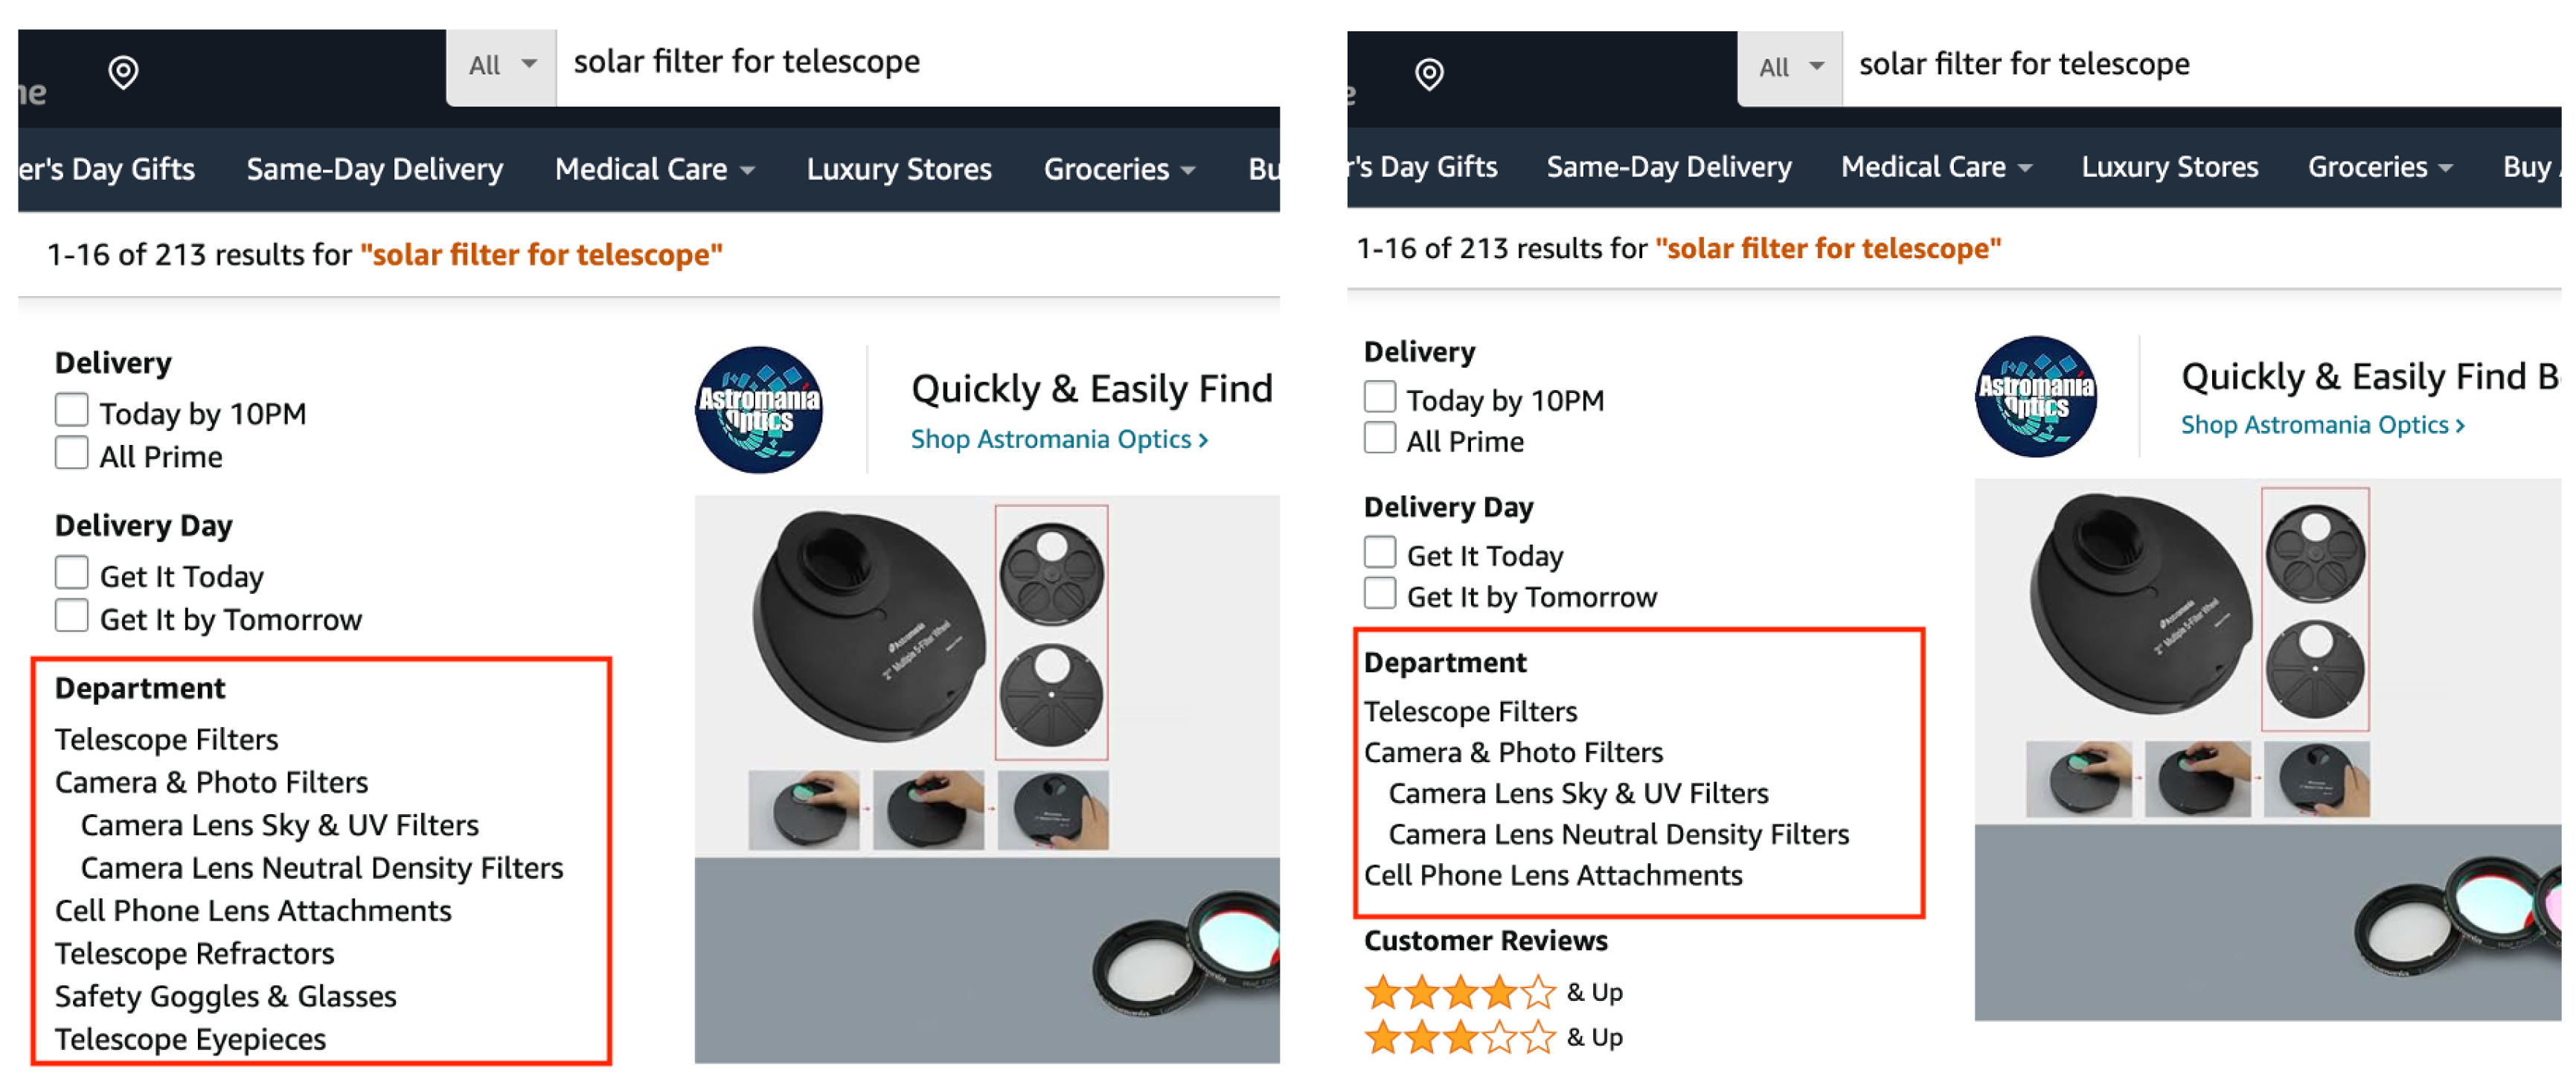
\includegraphics[width=.8\linewidth]{figures/agentab/filter_panel_design.png}
  \end{figure}
  \centering\small \textbf{Control}: full filter panel \quad vs.\quad \textbf{Treatment}: reduced panel (similarity ranking)\\
  \textbf{1,000} agents (500/condition) --- $\approx$10\% of a real A/B test.
\end{frame}

% ---- Results ----
\begin{frame}{Results: Reduced Filter $\rightarrow$ More Purchases}
  \begin{figure}[htp]
    \centering
    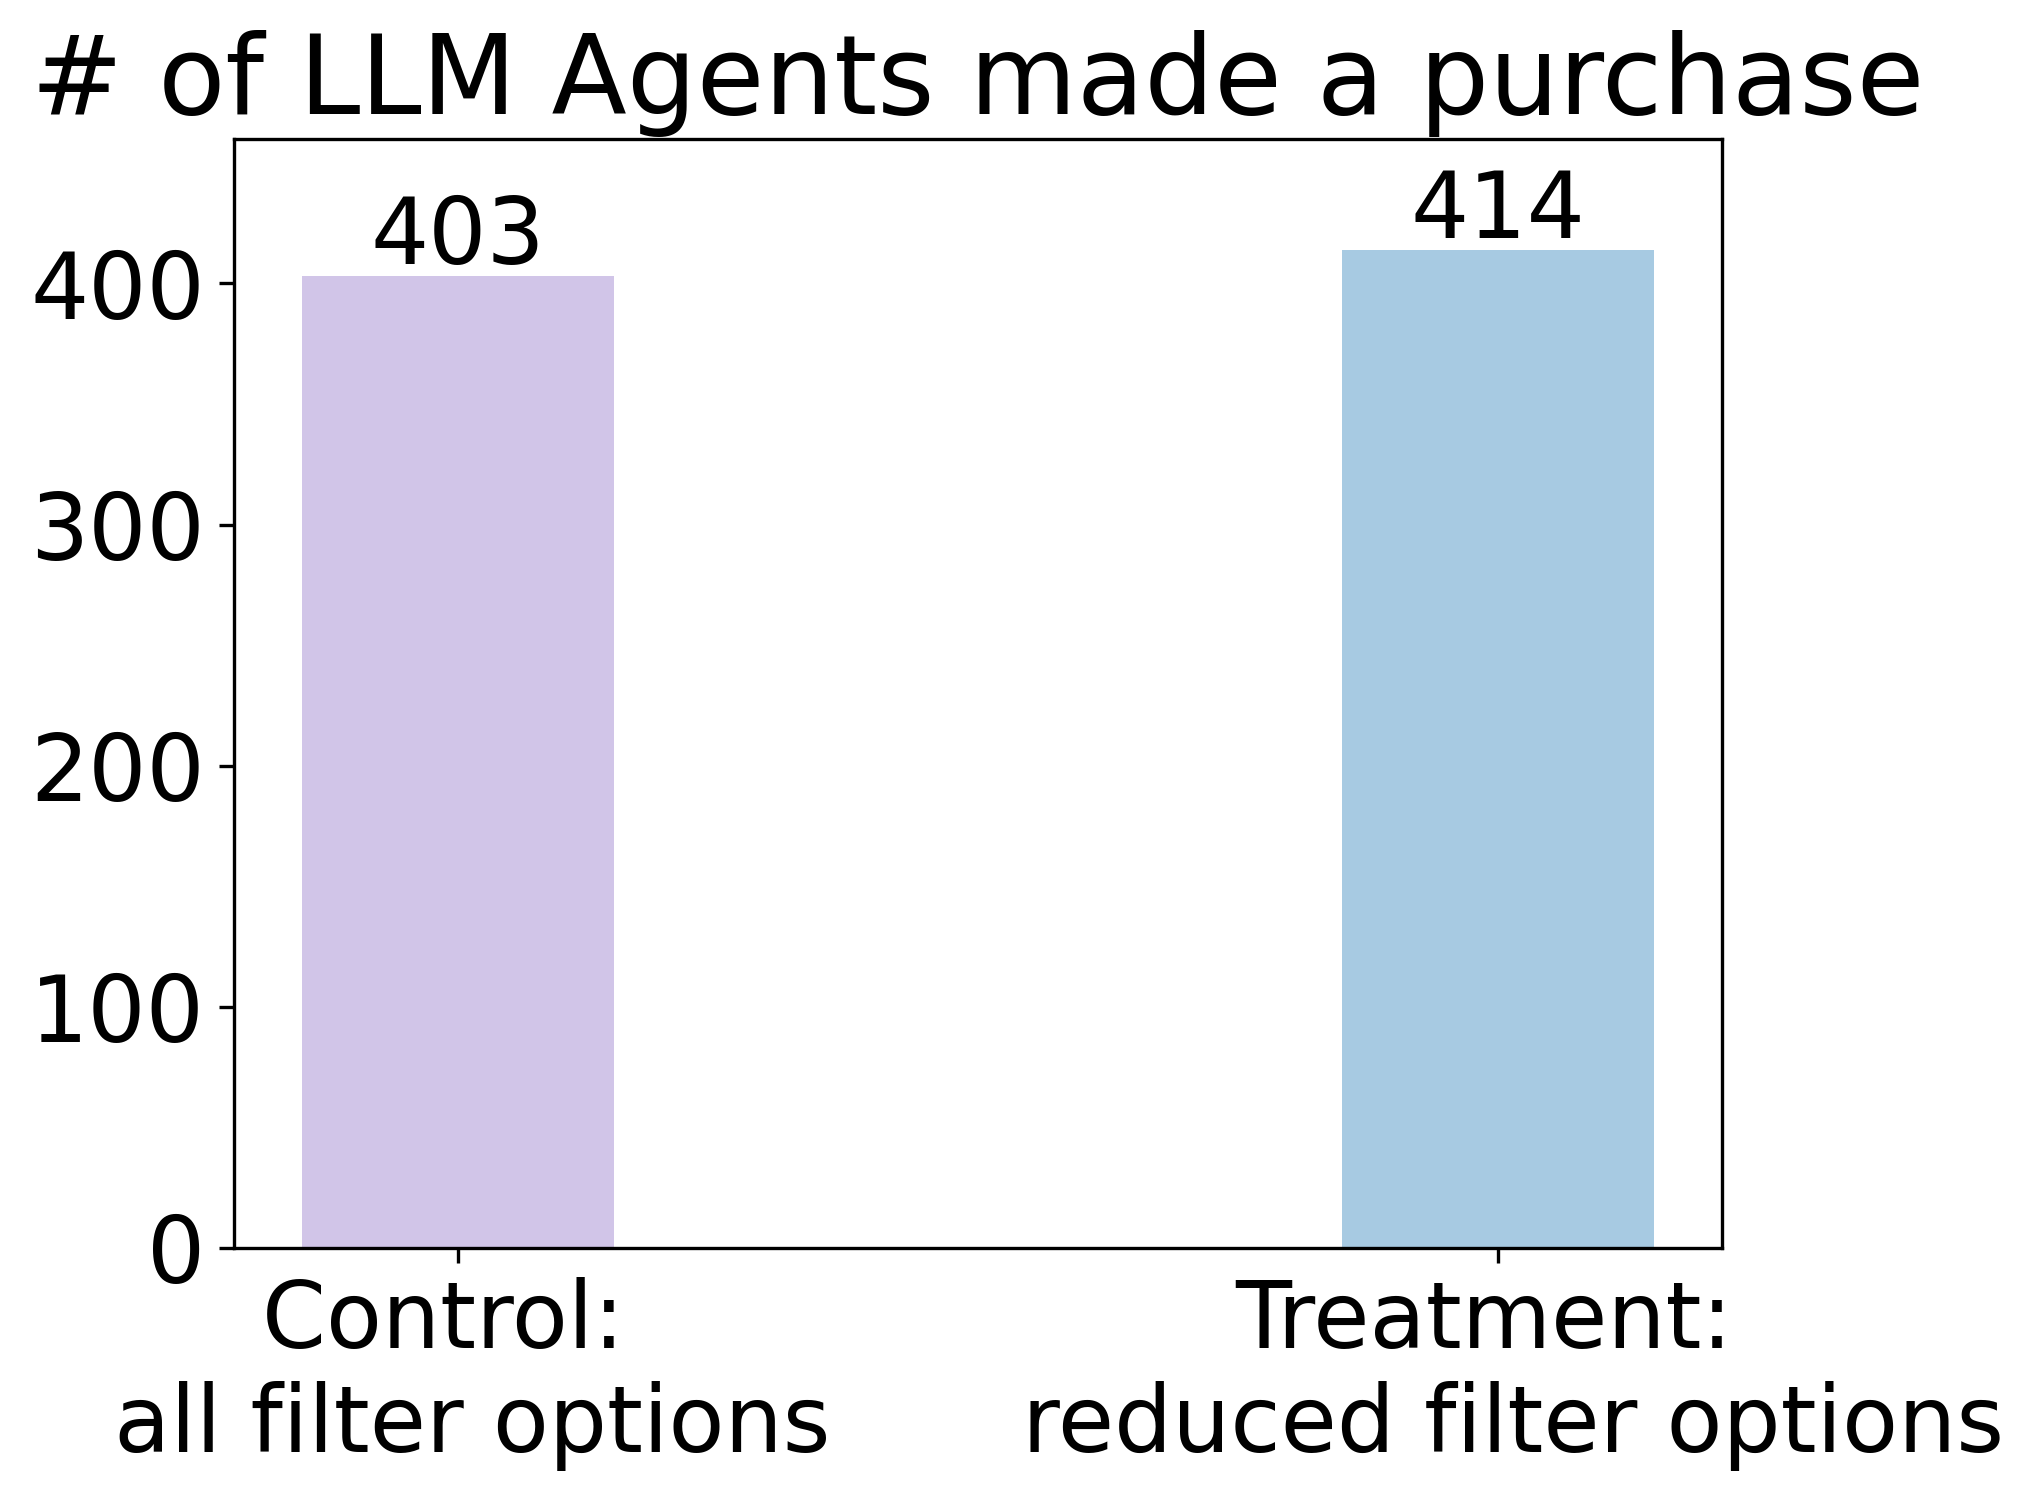
\includegraphics[width=.62\linewidth]{figures/agentab/bar.png}
  \end{figure}
  \centering\small \textbf{414 vs.\ 403} purchases --- a modest but statistically reliable increase.
\end{frame}

\begin{frame}{Subgroup Effects}
  \begin{columns}[c]
    \begin{column}{0.5\linewidth}
      \centering
      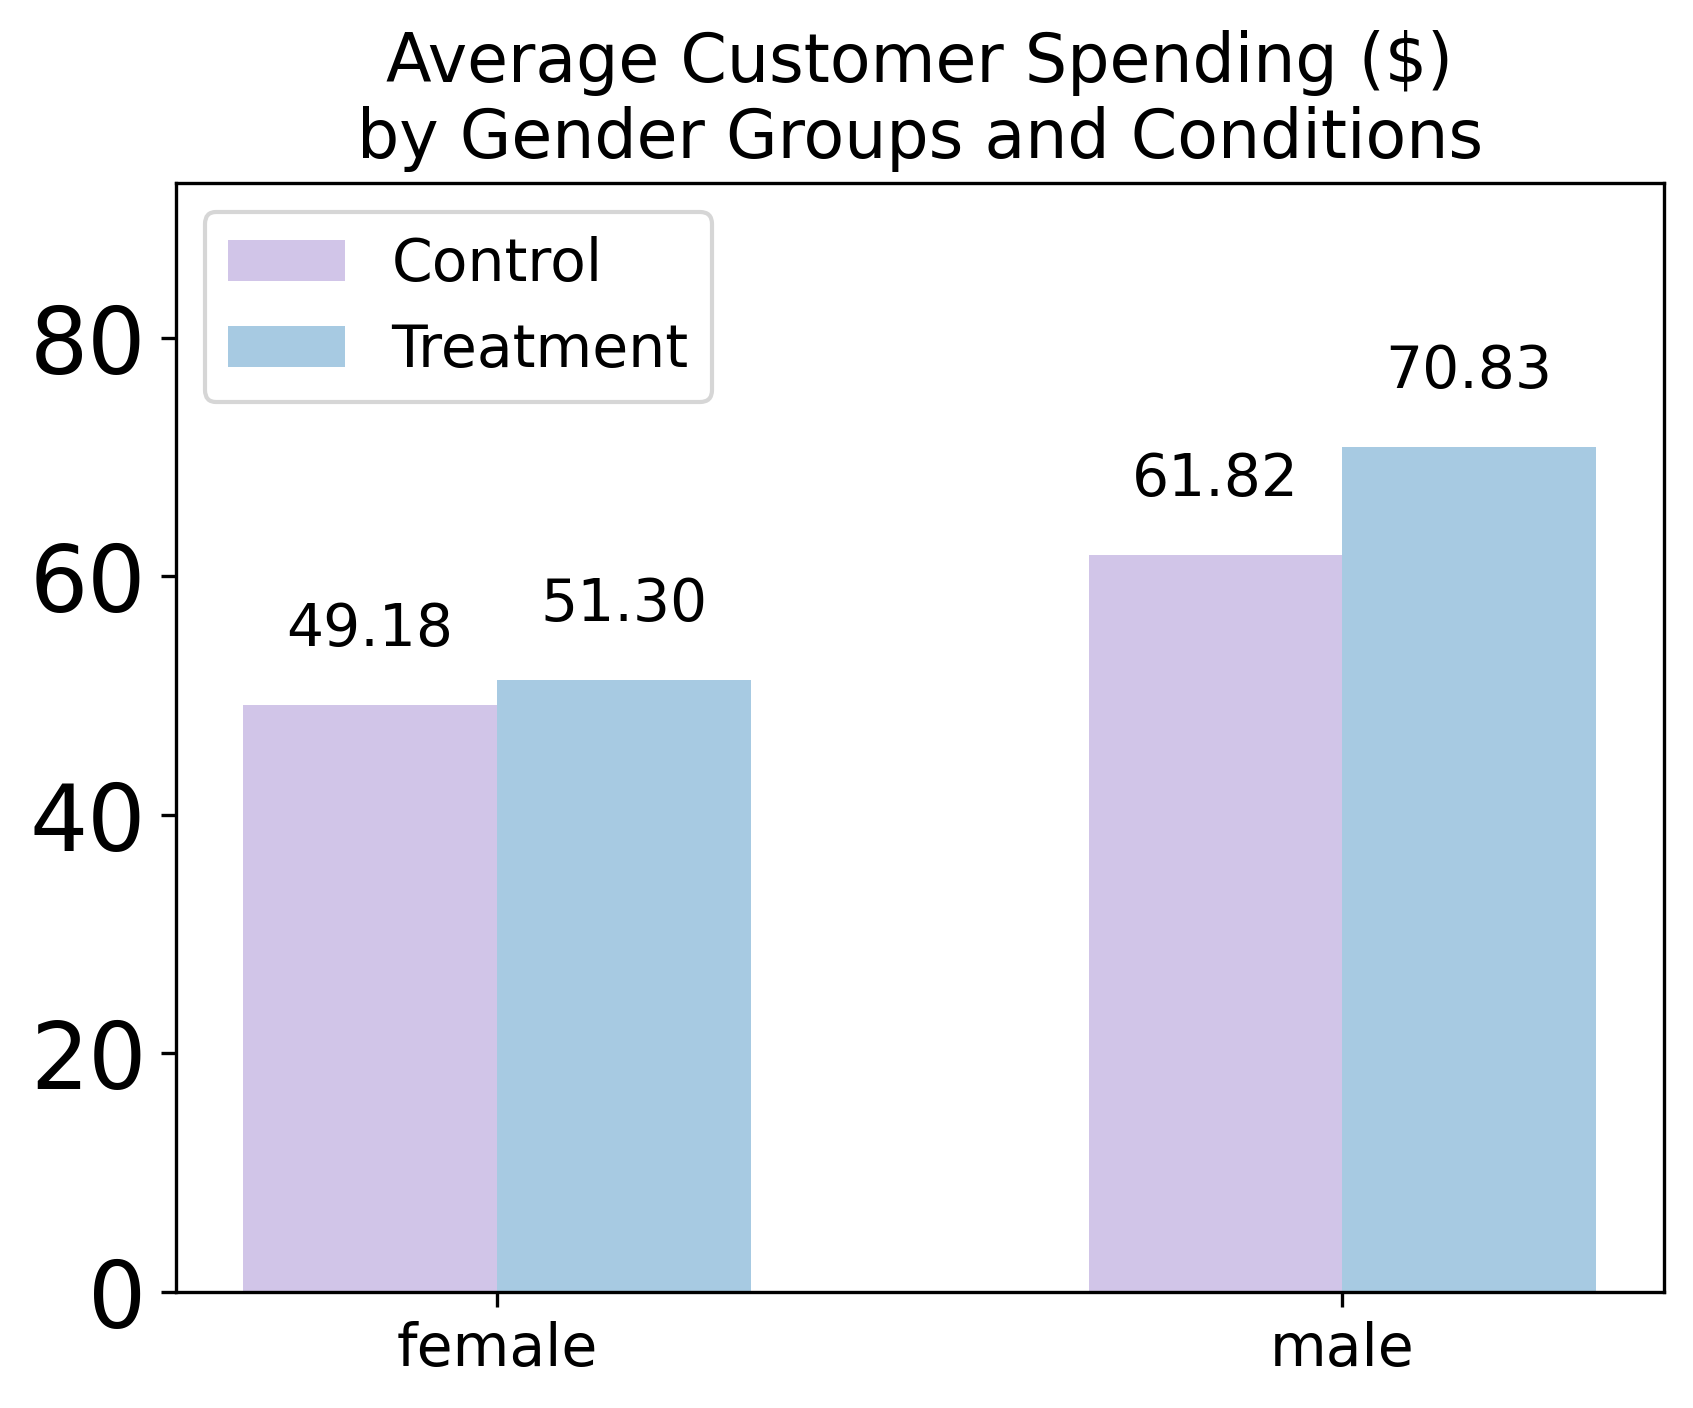
\includegraphics[width=\linewidth]{figures/agentab/control_treatment_gender_bar.png}
    \end{column}
    \begin{column}{0.5\linewidth}
      \centering
      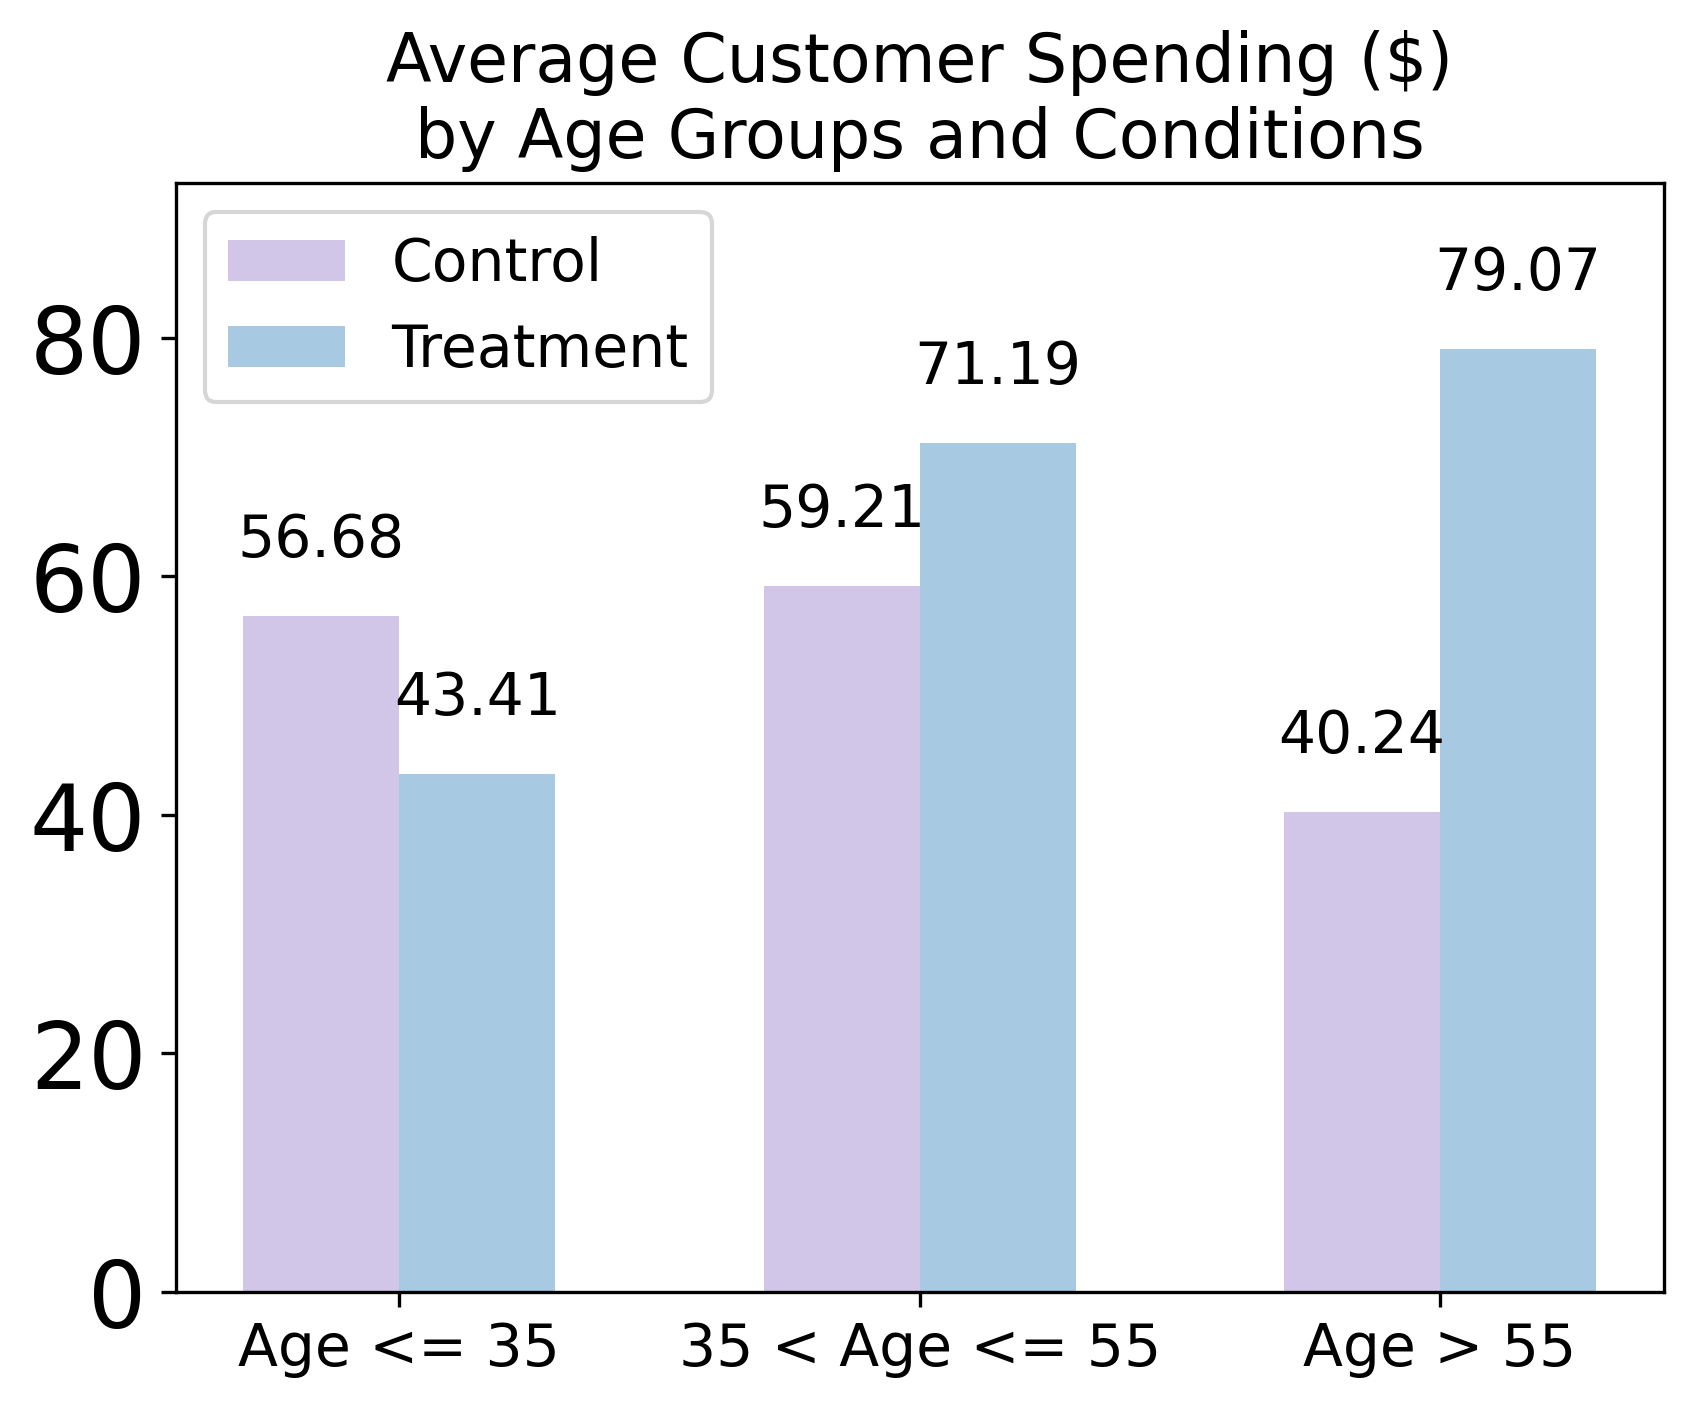
\includegraphics[width=\linewidth]{figures/agentab/control_treatment_age_bar.png}
    \end{column}
  \end{columns}
  \vspace{4pt}
  \centering\small Effects are stronger for \textbf{male} and \textbf{older} personas.
\end{frame}

% ---- Key validation ----
\begin{frame}[standout]
  Agent outcomes align \emph{directionally} with a parallel
  \textbf{large-scale human A/B experiment}.
\end{frame}

% ---- Handoff to Case Study 3 ----
\begin{frame}[standout]
  Simulated users can \ul{scale} --- \\ and point in the right direction.
  \vspace{10pt}
  \pause

  But ``directionally aligned'' $\neq$ ``accurate''.
  \vspace{4pt}

  \emph{How faithful are these agents, really?}
\end{frame}
